%%%%%%%%%%%%%%%%%%%%%%%%%%%%%%%%%%%%%%%%%%%%%%%%%%%%%%%%%%%%%%%%%%%%%%%%%%%%%%%%%%%%%%%%%%%%%%%%%%%%%%%%%%
\section{Introduction}\label{sec:introduction}


It is already a well-known fact that the type of traffic used on performing tests matters. Studies show that a realistic Ethernet traffic provides a different and more variable load characteristics on routers\cite{harpoon-validation}, even with the same mean bandwidth consumption. It indicates that tests with constant bit rate traffic generator tools are not enough for a complete validation of a new technology. There are many reasons for this behavior, which includes burstiness and packet sizes. A burstier traffic can cause packet more buffer overflows on network\cite{burstiness-queue-lenght}\cite{modelling-of-self-similar}\cite{empirical-interarrival-study}, degenerating network performance\footnote{Fuatures such as packet-trains periods and inter-packet times affect traffic burstiness}. Also, a burstier and realistic traffic will not just impact on performance, but on measurement as well, since a realistic and burstier traffic impacts on bandwidth measurement accuracy\cite{legotg-paper}\cite{background-traffic-matter}. Knowing that, many traffic generator tools\cite{ditg-paper} provide a set of pre-defined stochastic models to control the emission packets, controlling packet-trains and inter-pacekt times. 



There are many works devoted on studing the nature of the Ethernet traffic~\cite{selfsimilar-ethernet}\cite{analysis-self-similar}\cite{stochartic-selfsimilar}\cite{selfsimilar-highvariability}\cite{multi-player-online-game-self-similarity}. Classic Ethernet models use Poisson related processes, wich represents the probability of events occur in many independent sources with a known average rate, and independently of the last occurrence~\cite{selfsimilar-ethernet}~\cite{book-poisson}. However studies made by Leland et al.~\cite{selfsimilar-ethernet} showed that the Ethernet traffic has a self-similar and fractal nature. Even if they can represent the randomness of an Ethernet traffic, simple Poisson processes can't express traffic "burstiness" in a long-term time scale, such as traffic "spikes" on long-range ripples. These characteristics are an indication of the fractal and self-similar nature of the traffic that usually we express by distributions with infinite variance, called heavy-tailed. Heavy-tail means its distribution is not exponentially bounded\cite{sourcesonoff-paper}, such as Weibull, Pareto and Cauchy distribution.  Heavy-tailed processes may guarantee self-similarity, but not necessarily will ensure other important features like high correlation between data and same mean packet rate\cite{validate-trafficgen}. 


Therefore, there are many investigations on how to model stochastic functions for different scenarios~\cite{estimation-renewal-function-ethernet-traffic}\cite{modelling-of-self-similar}\cite{empirical-interarrival-study}\cite{modeling-concurrent-heavy-tailed}\cite{optimal-scheduling-of-heavy-tailed-traffic}\cite{modelling-of-self-similar}. However, there are some limitations on this idea of finding a single ideal model. Usually, not the same stochastic distribution will present a proper fitting for all possible kinds of traces~\cite{sourcesonoff-paper}. Depending on some variables, such as the capture time, the number of packets or type of traffic, different functions may fit better the available data. On most works the best model representation for an Ethernet traffic is not chosen analytically but based on the researcher own data analyses and purposes~\cite{hierarchical-dynamics-interarrival-times}\cite{modeling-concurrent-heavy-tailed}\cite{optimal-scheduling-of-heavy-tailed-traffic}. Also, some methods like linear regression may diverge sometimes. Furthermore, it has already been proven that a single model cannot represent arbitrary traffic traces~\cite{sourcesonoff-paper}.  



In this work we propose and evaluate the use of information criteria BIC (Bayesian information criterion) and AIC (Akaike information criterion) as tool for an automatic selection best fitting for inter-packet times of a traffic trace. It is an analytical and deterministic method which spares and avoid human analyzes, is easy to be implemented by software, and don't relies on simulations and generation of random data. We fit a set of stochastic models through different methods and applying BIC and AIC to choose the best.  



First, we explain the mathematical meaning of BIC and AIC and state the methods we are going to use to create a set of candidate models for our dataset. Then we define our cross-validation method based on a cost function $J$, attributing weights from the best to the worst representation for each properties using randomly generated data with our stochastic fittings, we can choose the best possible traffic model among these fittings. This cost function depends on important stochastic properties for traffic modelling. Thus we compare the results achieved by AIC/BIC and our cost function. In that way we show that thay are a worth method for inteligent selection of inter-packet times stochastic models, being able to gess models with smaller $J$ values. We also found that for traffic inter-packet times, that the difference between BIC and AIC values is minimal. Thus, selecting  one over the other does not seem a key question. 


%%%%%%%%%%%%%%%%%%%%%%%%%%%%%%%%%%%%%%%%%%%%%%%%%%%%%%%%%%%%%%%%%%%%%%%%%%%%%%%%%%%%%%%%%%%%%%%%%%%%%%%%%%
\section{Literature Review}\label{sec:review}

\subsection{Modelling Ethernet Traffic}

There are plenty of works on the literature which proposes new processes and methodologies for modeling times between packets and packet trains. Fiorini \cite{modeling-concurrent-heavy-tailed} presents a heavy-tailed ON/OFF model, which tries to represent a traffic generated by many sources. The model emulates a multiple source power-tail Markov-Modulated (PT-MMPP) ON/OFF process, where the ON times are power-tail distributed. They achieve analytical performance measurements using Linear Algebra Queueing Theory.

Kreban and Clearwater\cite{hierarchical-dynamics-interarrival-times} presents a model for times between job submissions of multiple users over a super computer. They show that the Weibull probability functions are able to express well small and high values of inter-job submission times. They also tested exponential, lognormal and Pareto distributions. Exponential distribution couldn't  represent long-range values because it fell off too fast and Pareto was too slow. Lognormal fit well small values, but was poor on larger ones. Kronewitter\cite{optimal-scheduling-of-heavy-tailed-traffic} presents a model of scheduling traffic of many heavy-tail sources. On his work, he uses many Pareto sources to represent the traffic. To estimate the shape parameter $\alpha$ they use linear regression.


\subsection{AIC and BIC}

Suppose that we have an statistical model $M$ of some dataset ${\boldsymbol{x} = \{x_1, ..., x_n}\}$, with $n$ independent and identically distributed observations of a random variable $X$. This model can be expressed by a probability density function (PDF) $f(x| \boldsymbol{\theta})$, where $\boldsymbol{\theta}$ is a vector of parameter of the PDF, $\boldsymbol{\theta} \in \mathbb{R}^{k}$ ($k$ is the number of parameters). The  likelihood function  of this model $M$ is given by:
\begin{equation}
L(\boldsymbol{\theta}|\boldsymbol{x} ) =  f(x_1|\boldsymbol{\theta})\cdot...\cdot f(x_n|\boldsymbol{\theta}) = \prod_{i = 1}^{n}f(x_i|\boldsymbol{\theta})
\end{equation}
Now, suppose we are trying to estimate the best statistical model, from a set ${M_1, ..., M_n}$, each one with an estimated vector of parameters  ${\boldsymbol{\hat{\theta_1}}}, ..., {\boldsymbol{\hat{\theta_n}}}$. $AIC$ and $BIC$ are defined by:
\begin{equation}
AIC = 2k - \ln(L(\boldsymbol{\hat{\theta}}|\boldsymbol{x}))
\end{equation}
\begin{equation}
BIC = k\ln(n) - \ln(L(\boldsymbol{\hat{\theta}}|\boldsymbol{x}))
\end{equation}
In both cases, the preferred model $M_i$, is the one with the smaller value of $AIC_i$ or $BIC_i$.

%%%%%%%%%%%%%%%%%%%%%%%%%%%%%%%%%%%%%%%%%%%%%%%%%%%%%%%%%%%%%%%%%%%%%%%%%%%%%%%%%%%%%%%%%%%%%%%%%%%%%%%%%%
\section{Methodology}


We start defining the \textit{pcaps} datasets we are going to use in the rest of this text. We will use for datasets, and for reproduction purposes, three are public available. 
The first is a lightweight Skype packet capture, found in  Wireshark wiki\footnote{ Available at \url{https://wiki.wireshark.org/SampleCaptures}, named  \textit{SkypeIRC.cap}}, we call it \textit{skype-pcap}. The second is a CAIDA\footnote{ \url{http://www.caida.org/home/} } capture, wich we analyze its first second capture\footnote{Available at \url{https://data.caida.org/datasets/passive-2016/equinix-chicago/20160121-130000.UTC}, named as \textit{equinix-chicago.dirB.20160121-135641.UTC.anon.pcap.gz}  }, and we refer to it as \textit{wan-pcap}. The third we capture in our laboratory LAN, through a period of 24 hours. It was captured firewall gateway between our local and external network. Along with other tests, We intend to verify diurnal behavior on it. That means a high demand of packets during the day and a small in the night. We call it \textit{lan-diurnal-pcap}. Finally, the last is a capture of a busy private network access point to the Internet, available on-line on TCPreplay website \footnote{Available at \url{http://tcpreplay.appneta.com/wiki/captures.html}, named \texttt{bigFlows.pcap}}, we will refer to it \textit{bigflows-pcap}.

Further we collect inter-packet times from the traffic traces. Then, we estimate a set of parameters for stochastic processes, using a set of different methodologies such as linear-regression, maximum likelihood, and direct estimation of parameters. We are modelling: 

\begin{itemize}
\item Weibull, exponential, Pareto and Cauchy distributions, using linear regression, through the Gradient descendent algorithm. We refer to these exponential and Pareto approximations as Exponential(LR) and Pareto(LR);
\item Normal and exponential distribution, using direct estimation the mean and the standard deviation of the dataset for the normal, and the mean for the exponential. We refer for to this exponential approximation as Exponential(Me);
\item Pareto distribution, using the maximum likelihood method. We refer to this distribution as Pareto(MLH);
\end{itemize}





Then, from these parametrized models, we estimate which one best represent our dataset, using AIC  and BIC criteria. These results were obtained using Octave language\footnote{ \url{https://www.gnu.org/software/octave/}}, and the scripts are available at \cite{projeto-github} for reproduction purposes. Thus, to see if our criterion of parameter selection can find which is the best model according to traffic modeling standards on realism and benchmarking\cite{validate-trafficgen}, we define a validation methodology. We randomly generated a dataset using our parameterized stochastic processes.  Moreover, we compare it with the original and synthetic sample, trough three different metrics, all with a confidence interval of 95\%:

\begin{itemize}
\item Correlation between the sample data and the estimated model (Pearson's product-moment coefficient);
\item Difference between the original and the synthetic Hurst exponent;
\item Difference between the original and the synthetic mean inter-packet time;
\end{itemize}

The Pearson's product-moment coefficient, or simply correlation coefficient,  is an expression of the dependence or association between two datasets. Its value goes from -1 to +1. +1 means a perfect direct linear correlation. -1 indicates perfect inverse linear correlation. 0 means no linear correlation. So, as close the result reach 1, more similar are the inter-packet times to the original values. To estimate it, we use the Octave's function \texttt{corr()}.

The Hurst exponent is meter self-similarity and indicates the fractal level of the inter-packet times. As close the result is from the original, more similar is the fractal level of the estimated samples from the original. To estimate this value we use the function \texttt{hurst()} from Octave, which uses rescaled range method. Finally, the mean is also relevant, since it will meters if the packet per second rate of the trace and its approximation model are close related. 

To quantitatively check   if AIC and BIC are good criteria for model selection for inter-packet times, we define a cost function based on the correlation, Hurst exponent and mean. We defined a cost function $J$, based on the randomly generated data values with our estimated stochastic process. Being $Cr$ the vector of correlations ordered from the greater to the smaller. Let $Me$ and $Hr$ defined by the absolute difference between mean and hurt exponent of the estimated values and the original dataset. Both are ordered from the smaller to the greatest values. Letting $\phi(V, M)$ be an operator who gives the position of a model $M$ in a vector $V$, we define the cost function $J$ as:

\begin{equation}
J(M) = \phi(Cr, M) + \phi(Me, M) + \phi(Hr, M)
\end{equation}

The smaller is the cost $J$, the best is the model. Then we compare the results achieved by AIC and BIC, and $J$.


%\begin{table*}[t]
%\centering
%\caption{Results of our modeling and simulation methodology for the traffic trace \textit{skype-pcap}. The stochastic processes are ordered form the worst to the best fitting, according to AIC and BIC.}
%\label{tab:skype-results}
%\begin{tabular}{lcccc}
%\hline
%Function        & AIC         & BIC        & \multicolumn{2}{c}{Parameters}      \\ \hline
%Weibull         & $-2293.8$   & $-2283.8$ & $\alpha:0.522$ & $\beta:0.097$  \\
%Exponential (Me) & $-426.13$   & $-421.1$  & \multicolumn{2}{c}{$\lambda:3.319$}  \\
%Exponential (LR) & $96.9$   & $101.8$  & \multicolumn{2}{c}{$\lambda:1.505$}         \\
%Pareto (MLH)     & $361.9$   & $371.8$  & $\alpha:0.0747$ & $x_m:5e-8$       \\
%Normal          & $2423.8$    & $2433.8$   & $\mu:0.301 $   & $\sigma:0.749$ \\
%Pareto (LR)      & $6411.0$   & $6421.1$  & $\alpha:0.413$ & $x_m:5e-8$       \\
%Cauchy          & $13464.6$    & $13474.5$   & $\gamma:0.000275$ & $x_0:0.219$    \\ \hline
%\end{tabular}
%\end{table*}

\begin{figure}[ht!]
{\centering
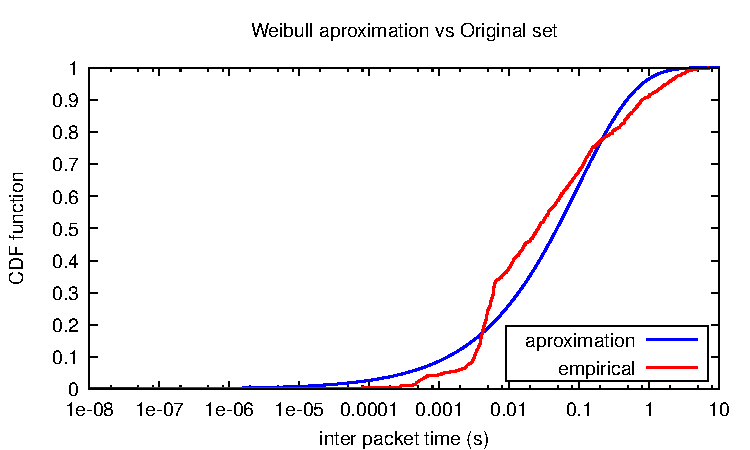
\includegraphics[width=\columnwidth]{figures/Weibull}
\caption{Cumulative distribution function(CDF) for Weibull fitting and empirical data for inter-packet times of \textit{skype-pcap}}
\label{fig:skype-weibull}\par}
\end{figure}

\begin{table*}[ht!]
	\centering
	\caption{Results of the octave prototype, include BIC and AIC values, para estimated parameters for two of our pcap traces: \textit{skype-pcap }and \textit{bigflows-pcap}. \textit{bigflows-pcap} is much larger, and has a much much smaller mean inter-packet time}
    \scalebox{0.95}{ 
		\begin{tabular}{lcccccccccc}
			\hline
			& \multicolumn{10}{c}{Trace} \\ \cline{2-11} 
			Function		& Order & AIC  & BIC  & \multicolumn{2}{c}{Parameters}  
			& Order & AIC & BIC  & \multicolumn{2}{c}{Parameters} \\ \hline 
			
			& \multicolumn{5}{c}{skype-pcap}  & \multicolumn{5}{c}{lan-diurnal-pcap}   \\ \hline 
			Cauchy          &	7 & $1.35e4$    & $2.19e4$    & $\gamma:2.59e-4$ & $x_0:1.05e-1$    
			&	5 & $-2.85e7$   & $-2.85e7$   & $\gamma:9.63e-3$ & $x_0:-3.61e-3$    \\
			Exponential(LR) &	3 & $9.69e1$   & $1.02e2$   & \multicolumn{2}{c}{$\lambda:1.86$}   
			&	6 & $1.79e6$    & $1.79e6$    & \multicolumn{2}{c}{$\lambda:8.51e-1$}    \\
			Exponential(Me) &	2 & $-4.26e2$   & $-4.28e3$   & \multicolumn{2}{c}{$\lambda:7.01$}   
			&	4 & $-3.12e7$   & $-3.12e7$   & \multicolumn{2}{c}{$ \lambda:58.78$} \\
			Normal          &	5 & $2.42e3$    & $3.31e3$    & $\mu:1.43e-1 $    & $\sigma:5.01e-1$ 
			&	7 & $Inf$       & $Inf$       & $\mu:1.70e-2$     & $\sigma:8.56e-2$ \\
			Pareto(LR)      &	6 & $6.4e3$   & $-8.27e3$   & $\alpha:2.52e-1$ & $x_m:5e-8$    
			&	3 & $-4.60e7$   & $-4.60e7$   & $\alpha:2.55e-1$ & $ x_m:5e-8$    \\
			Pareto(MLH)     &	4 & $3.62e2$   & $3.72e2$   & $\alpha:9.21e-2$ & $x_m:5e-8$    
			&	2 & $-5.03e7$   & $-5.03e7$   & $\alpha:1.15e-1$ & $ x_m:5e-8$    \\
			Weibull         &	1 & $-2.29e3$   & $-2.28e3$  & $\alpha:3.20e-1$ & $\beta:1.52e-2$  
			&	1 & $-5.60e7$   & $-5.60e7$   & $\alpha:3.34e-1$ & $\beta:1.83e-3$  \\ \hline	
			& \multicolumn{5}{c}{bigFlows-pcap} & \multicolumn{5}{c}{wan-pcap}  \\ \hline
			Cauchy          &	6 & $7.14e6$    & $7.14e6$   & $\gamma:1.94e0$ &$x_0:-7.25$    
			&	7 & $5.99e7$    & $5.99e7$   & $ \gamma:8.28e2$ &$x_0:-4.52e3$    \\
			Exponential(LR) &	7 & $7.33e6$    & $7.33e6$   & \multicolumn{2}{c}{$\lambda:1.489e-1$}   
			&	6 & $5.68e7$    & $ 5.68e7$  & \multicolumn{2}{c}{$\lambda:2.2e-5$}   \\
			Exponential(Me) &	2 & $-1.09e7$   & $-1.09e7$  & \multicolumn{2}{c}{$\lambda:2.64e3$}   
			&	1 & $-6.58e7$   & $-6.58e7$  & \multicolumn{2}{c}{$\lambda:6.58e5$} \\
			Normal          &	5 & $-9.35e6$   & $-9.35e6$  & $\mu:3.79e-4$   &$\sigma:6.60e-4$ 
			&	2 & $-6.39e7$   & $-6.39e7$  & $\mu:2e-6$     & $\sigma:1e-6$ \\
			Pareto(LR)      &	4 & $-1.02e7$   & $-1.02e7$  & $\alpha:1.489e-1 $ & $x_m:5e-8 $    
			&	4 & $-5.31e7$   & $-5.31e7$  & $\alpha:NaN$ & $x_m:5e-8 $    \\
			Pareto(MLH)     &	3 & $-1.03e7$   & $-1.03e7$  & $\alpha:1.362e-1$ & $x_m:5e-8 $    
			&	5 & $-6.25e7$   & $-6.25e7$  & $\alpha:3.39e-1$ & $x_m:5e-8 $    \\
			Weibull         &	1 & $-1.10e7$   & $-1.10e7$  & $\alpha:2.81e-1$ & $\beta:5.54e-4$  
			&	3 & $-5.46e7$   & $-5.46e7$  & $\alpha:7.64e-2$ & $\beta:1e-6$  \\ \hline
		\end{tabular}
        }
	\label{tab:prototype-results}
\end{table*}

\begin{figure}[ht!]
{\centering
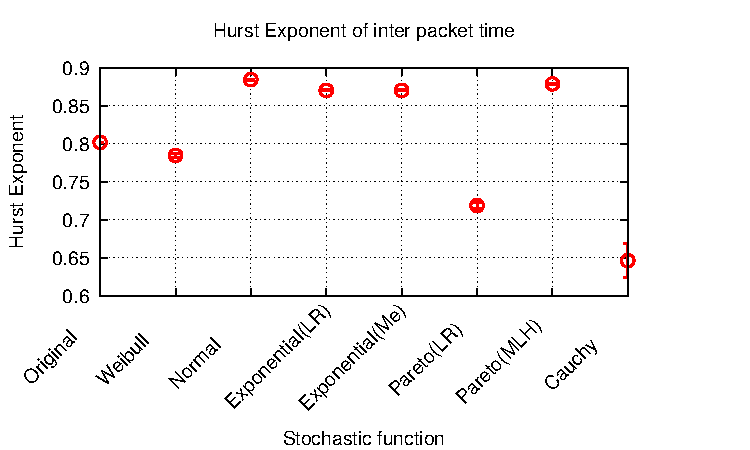
\includegraphics[width=\columnwidth]{figures/Skype_Hurst_Exponent}
\caption{Hurst exponent calculation of inter-packet times for \textit{skype-pcap} and its approximations}
\label{fig:skype-hurst}\par}
\end{figure}

\begin{figure}[ht!]
{\centering
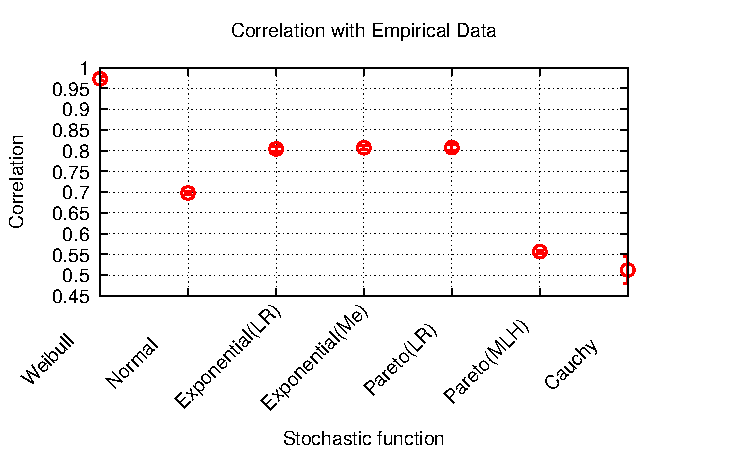
\includegraphics[width=\columnwidth]{figures/Skype_Correlation}
\caption{Correlation between \textit{skype-pcap} inter-packet times and its approximations.}
\label{fig:skype-correlation}\par}
\end{figure}

\begin{figure}[ht!]
{\centering
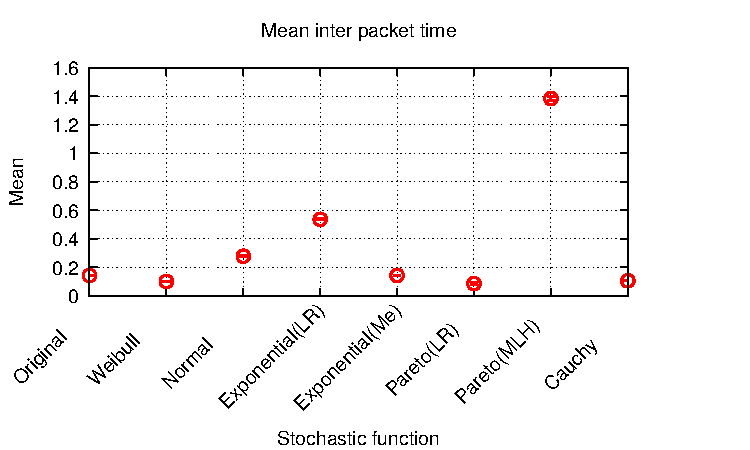
\includegraphics[width=\columnwidth]{figures/Skype_Mean}
\caption{Mean inter-packet times for \textit{skype-pcap} and its approximations.}
\label{fig:skype-mean}\par}
\end{figure}


\begin{figure*}[ht!]
	\centering
	\subfloat[\textit{skype-pcap}]{
		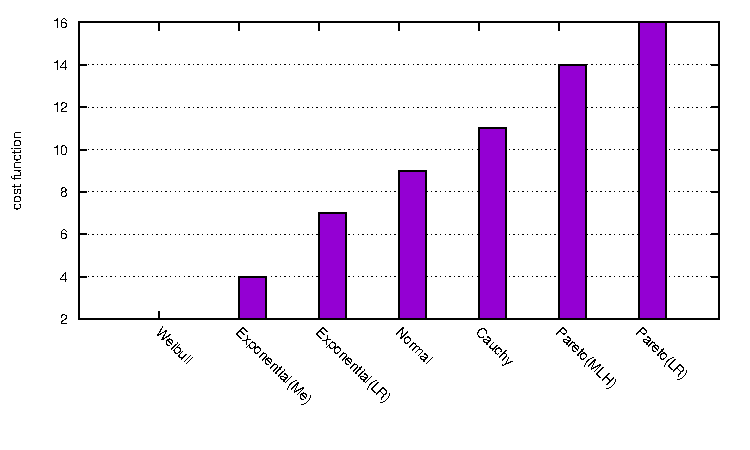
\includegraphics[width=75mm]{figures/Skype_costFunction}
		\label{cost-skype-pcap}
	}
	\hspace{0mm}
	\subfloat[\textit{bigFlows-pcap}]{
		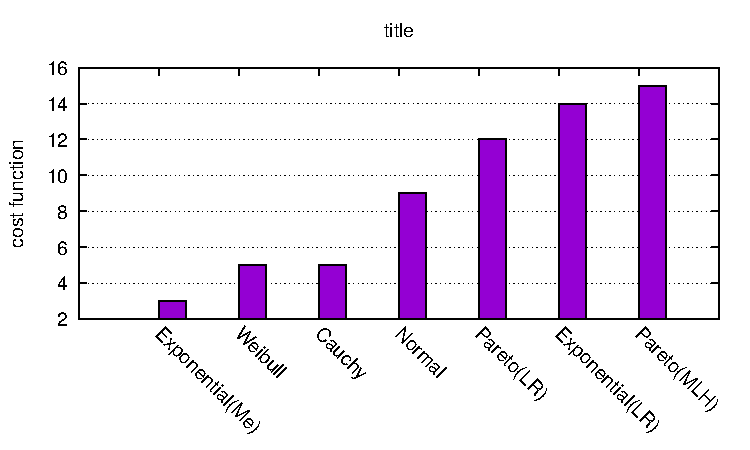
\includegraphics[width=75mm]{figures/bigFlows_costFunction}
		\label{cost-bigFlows-pcap}
	}
	\hspace{0mm}
	\subfloat[\textit{lan-diurnal-pcap}]{
		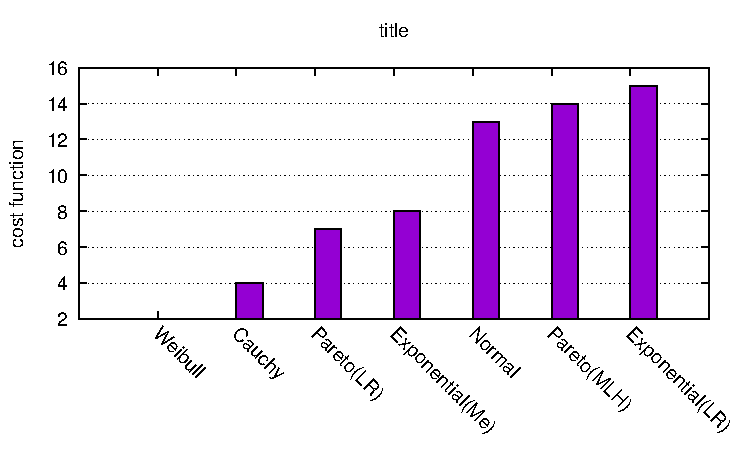
\includegraphics[width=75mm]{figures/Lan_costFunction}
		\label{cost-lan-pcap}
	}
	\hspace{0mm}
	\subfloat[\textit{wan-pcap}]{
		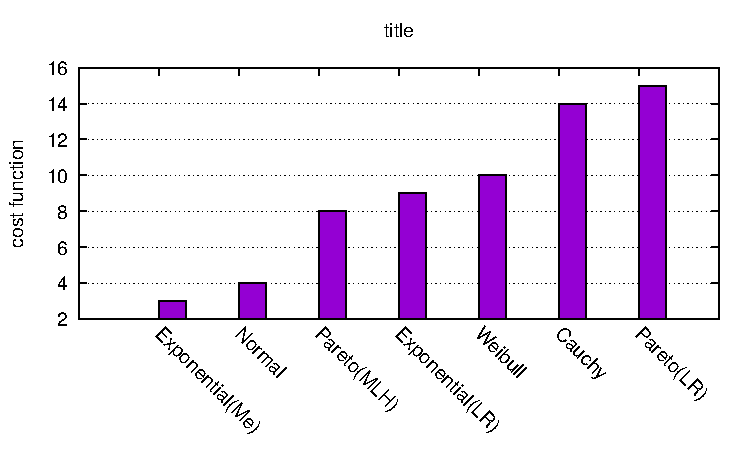
\includegraphics[width=75mm]{figures/Wan_costFunction}
		\label{cost-wan-pcap}
	}
	\caption{Cost function for each one of the datasets used in this validation process}
	\label{fig:cost-function}
\end{figure*}



\begin{figure}[ht!]
{\centering
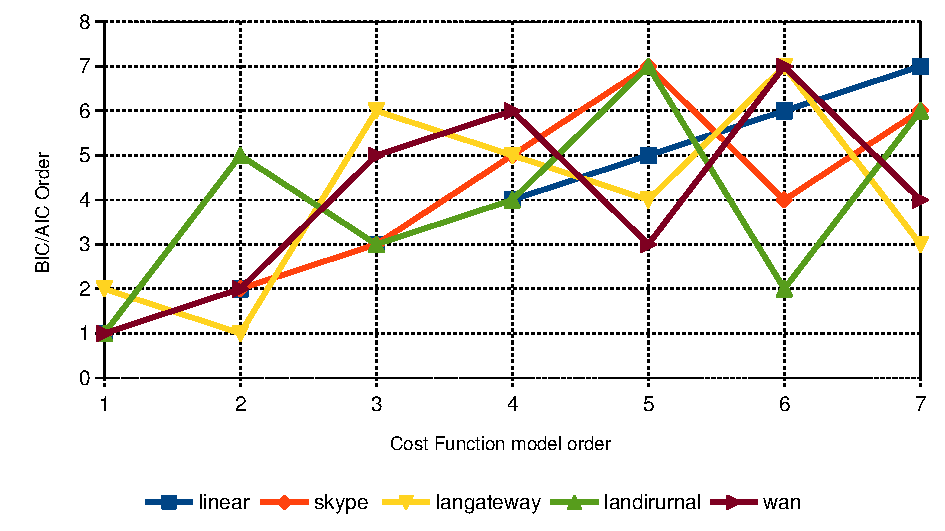
\includegraphics[width=\columnwidth]{figures/pcap-comparision}
\caption{Comparision of the model selection order for BIC/AIC and the cost function for each pcap.}
\label{fig:model-order}\par}
\end{figure}

%Analyzing the plots, and what they would mean, our Cauchy fitting would impose an almost contant traffic , with the inter packet time close to the mean. On the trace \textit{skype-pcap} the exponential plots seems to not represent well the small values of inter packet times. This is due fact that an exponential process is good at representing values close to the mean. But, it fails to represent values too small and higher. On the other hand, a self-similar process like Weibull and Pareto are better representing inter packet times with higher dispersion. Pareto(MLH) has a slow convergence, wich means this distribution may genarate values of inter-packet times too large. 

%Analyzing the QQplots, we may observe that in most of the distribution, the samples (original data) has a much havier-tail effect than in the estimated data. This is verified by the almost blue horizontal lines formed by the "exes". But, the Weibull distribution follow much closer the original data. Also is possible to see that the sample has a right skew compared to the estimation on Exponential(LR), Exponential(Me), Normal, and Pareto(MLH). This means that this estimation would not represent so well small values of time in this case. On the other hand, Pareto(LR) and Weibull would not suffer from this problem.

%The results for the AIC, BIC and parameters of all four traces are at the table~\ref{tab:prototype-results}.  The results for \textit{wan-pcap} and \textit{lan-diurnal-pcap} are on the table ~\ref{tab:prototype-results}. The difference between BIC and AIC values in all simulations are very small. Much smaller then the difference of these values between the distributions. This is an indication that for inter packet times, using AIC or BIC should will not influence significantly the results. 

%On our previsions, Weibull and Pareto(MLH and LR) are the best options. This was expected, since both are heavy-tailed functions. But Cauchy on most of the tests, even being a heavy-tailed distribution, seems to no present a good fitting. This is effect of the fast divergence of tangent function, when we linearize our data. 

%Analyzing the quality of AIC and BIC as criterion of choose on \textit{skype-pcap},based on the results form figure ~\ref{fig:correlation-hurst-skype-pcap} we see that in therms of Correlation and Self-similarity it picket the right model: Weibull. Also in therms of mean packet rate and dispersion it is still one of the best choises (along with Exponential(Me), Pareto(LR) and Cauchy). The third and the fourth choices (Pareto(LR)) and Exponential(LR) also are good options in most of these metrics. But, Pareto(MLH) is presented as the second best choice, and it had poor results in comparison to the others, especially on mean, correlation and dispersion. 

%All these results are abstracted by the cost function $J$. As we can see, on all pcaps, the best function selected by BIC and AIC~\ref{tab:prototype-results} also had the small cost~\ref{fig:cost-function}. 

%Another important observation is the fact that exponential function was able to provide the best fitting for the \textit{wan-pcap}. The reasons for this behavior are both result of a much intense traffic with no long-range gaps, and the precision of the measurement.



%%%%%%%%%%%%%%%%%%%%%%%%%%%%%%%%%%%%%%%%%%%%%%%%%%%%%%%%%%%%%%%%%%%%%%%%%%%%%%%%%%%%%%%%%%%%%%%%%%%%%%%%%%
\section{Results}


%Here in this chapter we only discuss the plots achived obtained by the pcap \textit{skype-pcap} for simplicity. The other plots are provided and commented on the appendix ~\ref{ap:aditional-plots}. In the figure ~\ref{fig:aproximation-original-cdf} we present all estimated CDF functions along with the empirical CDF, for the trace \textit{skype-pcap}. They are on logscale, wich provide a better visualization for small time scales. In the case of the normal function, all values smaller than zero, were set to zero on the plot. Is possible to see different accuracies and types of fittings on each plot. Visually, the best fit seems to be the Weibull trough linear regression. 





In table~\ref{tab:prototype-results} we summarize our estimations for AIC, BIC, and the stochastic process estimated parameters for all \textit{pcap} traces. We iserted and aditional column to facilitate the observation of the quality of fitting according BIC and AIC. For visualization, in the figure ~\ref{fig:skype-weibull} we present the best fitting chosen by BIC and AIC criteria for the \textit{skype-pcap}. It is on log-scale, which provides a better visualization for small time values. Visually we can see that linear regression with Weibull distribution was able to provide a good approximation for this dataset.

First, let's take a look on table ~\ref{tab:prototype-results}. On \textit{skype-pcap} and \textit{bigFlows-pcap}, \textit{lan-diurnal-pcap}, the fitting pointed as the best was Weibull, except on the \textit{wan-pcap}, where Exponential(Me) was selected. This can be explained by the fact that this one had the largest bandwidth from all three pcaps, having smaller inter-packet times with a smaller range, and closer to the mean. The difference between BIC and AIC values in all simulations is much smaller than the difference between each distribution (for most of the cases are not larger than 1\%). This result indicates that for inter-packet times, using AIC or BIC to pick a model, do not influence the results significantly.


For \textit{skype-pcap}, according to BIC and AIC previsions, Weibull and Exponential (Me and LR) are the best options, and the cost functions gave exact this same order~\ref{fig:cost-function}. In fact, Weibull pointed as the best stochastic function by BIC and AIC, has half of the penalty imposed by the cost function $J$. The following models however are not in the same order since some results are flipped. But still, no opposite correspondence can be found. No result found by AIC and BIC were far from the one pointed by $J$.  


Furthermore, for \textit{wan-pcap} and \textit{lan-diurnal-pcap}, the function pointed by AIC/BIC was the same as pointed by $J$: Exponential(Me) and Weibull respectivally. On \textit{big-Flows-pcap} the first two gesses values are flipped, however we can notice that the difference between the AIC/BIC values were of just 7\%, wich indicate a closer level of quality. A more complete chart of the selection order between both metricas are on the figure ~\ref{fig:model-order}, relative to the $J$ selection order. The linear patern represent the ideal results. In some cases, like the 2nd and 6th


%\begin{figure}[h]
%{\centering
%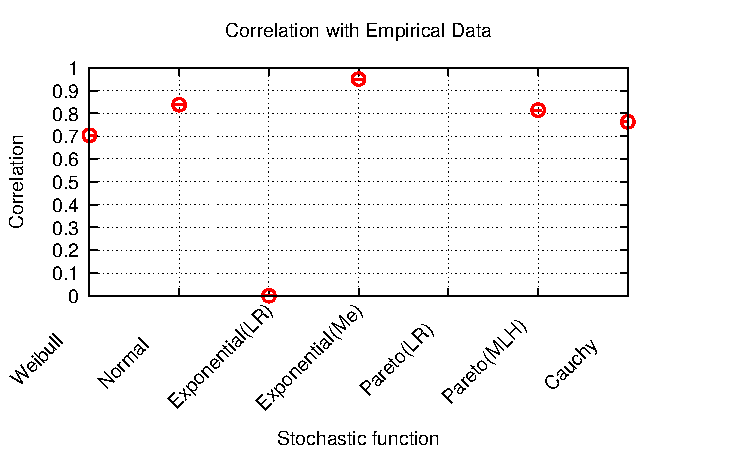
\includegraphics[width=\columnwidth]{figures/Correlation}
%\caption{Comparison between correlation of the used set of fittings, with a confidence of 95\%}
%\label{fig:skype-correlation}\par}
%\end{figure}


%\begin{figure}[t]
%{\centering
%\includegraphics[width=\columnwidth]{figures/HurstExponent}
%\caption{Comparison between the Hurst exponent of our approximated processes and the original data  with a confidence of 95\%}
%\label{fig:skype-hurst}\par}
%\end{figure}





%\begin{figure}[t]
%{\centering
%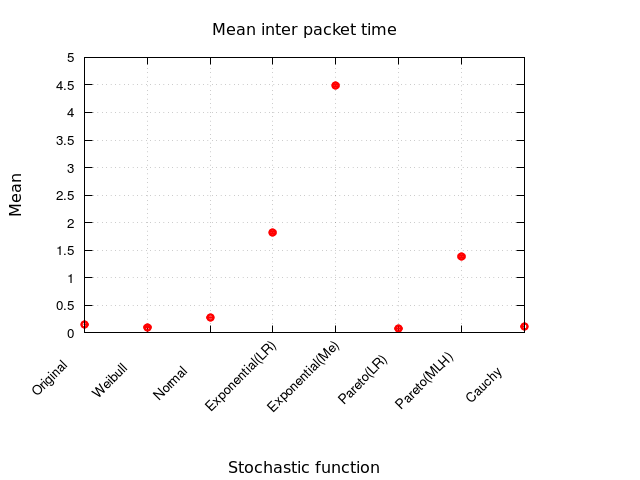
\includegraphics[width=\columnwidth]{figures/Mean}
%\caption{cap}
%\label{fig:skype-mean}\par}
%\end{figure}





%The difference between BIC and AIC values in all simulations are very small. Much smaller then the difference of these values between the distributions. This is an indication that for inter packet times, using AIC or BIC to pick a model, will not influence significantly the results. 

%According to BIC and AIC previsions, Weibull and Pareto(MLH and LR) are the best options. This was expected, since both are heavy-tailed functions. But Cauchy on most of the tests, even being a heavy-tailed distribution, seems to do no present a good fitting. This is effect of the fast divergence of tangent function, when we linearize our data. 

%From the figures ~\ref{fig:skype-correlation} and ~\ref{fig:fig:skype-hurst} we see that in therms of Correlation and Self-similarity it picket clearly the most related model: Weibull. Also in therms of mean packet rate it is still a good choice (along with Exponential(Me), Pareto(LR) and Cauchy). The third and the fourth choices (Pareto(LR)) and Exponential(Me) also are good options in most of these metrics. But, Pareto(MLH) is presented as the second best choice, and it had poor results in comparison to the others, especially on mean and correlation. This is the only model presented as good

%All these results are abstracted by the cost function $J$. As we can see, on all pcaps, the best function selected by BIC and AIC~\ref{tab:prototype-results} also had the small cost~\ref{fig:cost-function}. 

%Another important observation is the fact that exponential function was able to provide the best fitting for the \textit{wan-pcap}. The reasons for this behavior are both result of a much intense traffic with no long-range gaps, and the precision of the measurement.


\section{Conclusion}

In this work, we analyze how BIC and AIC perform being used as analytical selection criteria form stochastic models for Ethernet inter-packet times. Using a cross-validation methodology based on the generation of random data using these models, and pointing a cost function. We saw that both AIC or BIC and the cost function were able to pick the first models in the same order. Therefore, analytically with BIC and AIC, we were able to achieve the same results as pointed by our simulations. Even if AIC and BIC mathematical definitions are unaware of the specific requirements of Ethernet traffic modeling, such as same fractal-level and close packet per second rate, they still can point the best choices according to these constraints. 

In this work, we analyze just inter-packet times of a single trace. However at \cite{projeto-github} we perform the same methodology on different types of traffic captures, finding similar results. Therefore, we can conclude that BIC and AIC are healthy alternatives for model selection of Ethernet inter-packet times models and we can safely use them. Finally, we must point some advantages of BIC and AIC instead of simulations. Since it is an analytical model, no generation of random data is necessary,  being computationally cheaper and easy to code. Also, since we do not use a single stochastic function and parameterization strategy, it is resilient to the fact that some methods like linear-regression over Weibull may diverge sometimes. If it happens, BIC or AIC will discard this guesses, and choose another oneautomatically.

Last but not least, to the best of our knowledge, this is the most comprehensive investigation of the actual quality of BIC and AIC as model selection criteria of for inter-packet times.
%Also, except by the Pareto function modeled using the Maximum likelihood method, have comparative results between the simulations and the AIC/BIC goes. The best fittings according to the AIC/BIC usually returned very accurate models, with a small error between the mean and fractal level, and correlation close to one. The models selected as the worsts usually returned poor results.

%Also, it is important to notice that in some cases, some stochastic functions may perform poorly, and in other provide an accurate fitting, what justify the application of the criteria in all new experiments. For example, Weibull usually performs pretty well, but in some cases, perform poorly, and in others may even diverge. 

%We do not rely on only one type of parameterization. This turns our methodology more robust, since a linear regression may diverge. But always there will be a peaceable model, since our estimations for Normal, Exponential (Me) and Pareto (MLH) cannot. Models which the linear regression diverges, will have very high and positive BIC/AIC estimations, and will not stand as primary options.



